% --- INICIO DE PLANTILLA PERSONALIZADA ---
\documentclass[oneside,11pt]{Latex/Classes/PhDthesisPSnPDF}

% --- Paquetes Originales ---
\usepackage{blindtext}
\usepackage{actuarialangle} 
\usepackage{tabularx}
\usepackage{float}
\usepackage{multirow, array}
\usepackage[usenames,dvipsnames,svgnames,table]{xcolor}
\usepackage{longtable}
\usepackage{latexsym,amsmath,amssymb,amsfonts}
\usepackage{enumitem}
\usepackage{xparse}
\usepackage{booktabs}
\usepackage[round, sort, numbers]{natbib}  
\usepackage{adjustbox}
\usepackage[utf8]{inputenc}
\usepackage{caption}
\usepackage{graphicx}
\usepackage{hyperref}
\usepackage{cleveref}

% Definición de colores
\definecolor{miblue}{RGB}{68, 114, 196}

% --- CAMBIO CRÍTICO 1: Usar \input para macros en el preámbulo ---
% \include da problemas antes del begin document. \input es seguro.
% This file contains macros that can be called up from connected TeX files
% It helps to summarise repeated code, e.g. figure insertion (see below).

%%%%%%%%%%%%%%%%%%%%%%%%%%%%%%%%%%%%%%%%%%%%%%
%            Colores de la UNAM              %
%%%%%%%%%%%%%%%%%%%%%%%%%%%%%%%%%%%%%%%%%%%%%%
%Azul Pantone 541  -->(0,63,119) RGB
\definecolor{Azul}{RGB}{128,0,0}

%Oro Pantone 460  -->(234,221,150) RGB
\definecolor{Oro}{RGB}{234,221,150}


%%%%%%%%%%%%%%%%%%%%%%%%%%%%%%%%%%%%%%%%%%%%%%
%            Comandos para líneas            %
%%%%%%%%%%%%%%%%%%%%%%%%%%%%%%%%%%%%%%%%%%%%%%
%Se define un comando \colorvrule para hacer líneas verticales de color con 3 argumentos: color, ancho, alto
\newcommand{\colorvrule}[3]{
\begingroup\color{#1}\vrule width#2 height#3
\endgroup}

%Se define un comando \colorhrule para hacer líneas horizontales de color con 2 argumentos: color, ancho
\newcommand{\colorhrule}[2]{
\begingroup\color{#1}\hrule height#2
\endgroup}

%%%%%%%%%%%%%%%%%%%%%%%%%%%%%%%%%%%%%%%%%%%%%%
%          Comando para derivadas            %
%%%%%%%%%%%%%%%%%%%%%%%%%%%%%%%%%%%%%%%%%%%%%%
\newcommand{\derivada}[3][]{\ensuremath{\dfrac{\mbox{d}^{#1}#2}{\mbox{d}#3^{#1}}}} 
%primer argumento(opcional): orden de la derivada
%segundo argumento: función a derivar
%tercer argumento: variable respecto a la que se deriva


%%%%%%%%%%%%%%%%%%%%%%%%%%%%%%%%%%%%%%%%%%%%%%
%       Comando para la exponencial          %
%%%%%%%%%%%%%%%%%%%%%%%%%%%%%%%%%%%%%%%%%%%%%%
\newcommand{\e}[1][]{\ensuremath{\mbox{e}^{#1}}}
%primer argumento(opcional): exponente de la exponencial




% insert a centered figure with caption and description
% parameters 1:filename, 2:title, 3:description and label
\newcommand{\figuremacro}[3]{
	\begin{figure}[htbp]
		\centering
		\includegraphics[width=1\textwidth]{#1}
		\caption[#2]{\textbf{#2} - #3}
		\label{condicion}
	\end{figure}
}

% insert a centered figure with caption and description AND WIDTH
% parameters 1:filename, 2:title, 3:description and label, 4: textwidth
% textwidth 1 means as text, 0.5 means half the width of the text
\newcommand{\figuremacroW}[4]{
	\begin{figure}[htbp]
		\centering
		\includegraphics[width=#4\textwidth]{#1}
		\caption[#2]{\textbf{#2} - #3}
		\label{#1}
	\end{figure}
}

% inserts a figure with wrapped around text; only suitable for NARROW figs
% o is for outside on a double paged document; others: l, r, i(inside)
% text and figure will each be half of the document width
% note: long captions often crash with adjacent content; take care
% in general: above 2 macro produce more reliable layout
\newcommand{\figuremacroN}[3]{
	\begin{wrapfigure}{o}{0.5\textwidth}
		\centering
		\includegraphics[width=0.48\textwidth]{#1}
		\caption[#2]{{\small\textbf{#2} - #3}}
		\label{#1}
	\end{wrapfigure}
}

% predefined commands by Harish
\newcommand{\PdfPsText}[2]{
  \ifpdf
     #1
  \else
     #2
  \fi
}

\newcommand{\IncludeGraphicsH}[3]{
  \PdfPsText{\includegraphics[height=#2]{#1}}{\includegraphics[bb = #3, height=#2]{#1}}
}

\newcommand{\IncludeGraphicsW}[3]{
  \PdfPsText{\includegraphics[width=#2]{#1}}{\includegraphics[bb = #3, width=#2]{#1}}
}

\newcommand{\InsertFig}[3]{
  \begin{figure}[!htbp]
    \begin{center}
      \leavevmode
      #1
      \caption{#2}
      \label{#3}
    \end{center}
  \end{figure}
}







%%% Local Variables:
%%% mode: latex
%%% TeX-master: "~/Documents/sofia/Tesis Marines"
%%% End:


% --- Definiciones de seguridad (por si la clase falla al cargar alguna variable) ---
\providecommand{\facultad}[1]{\def\lafacultad{#1}}
\providecommand{\escudofacultad}[1]{\def\elescudo{#1}}
\providecommand{\degree}[1]{\def\elgrado{#1}}
\providecommand{\director}[1]{\def\eldirector{#1}}
\providecommand{\lugar}[1]{\def\ellugar{#1}}
\providecommand{\degreedate}[1]{\def\lafecha{#1}}

% --- Configuración para bloques de código de R (Pandoc) ---

%%%%%%%%%%%%%%%%%%%%%%%%%%%%%%%%%%%%%%%%%%%%%%%%%%%%%%%%%%%%%%%%%%%%%%%%%%%%%%%%
%                         DATOS (Conectados a RMarkdown)                       %
%%%%%%%%%%%%%%%%%%%%%%%%%%%%%%%%%%%%%%%%%%%%%%%%%%%%%%%%%%%%%%%%%%%%%%%%%%%%%%%%
\title{El análisis de datos en el comercio}
\author{Jeremías Mogollón \\ Hilary Andrade \\ Ronald Camacho \\ Angel
Mogollón}

% Lógica para Facultad: Si la defines en el YAML la usa, si no, usa la default

\facultad{Facultad de Ciencias Económicas y Sociales \\ Escuela de
Estadistica y Ciencias Actuariales}
  \escudofacultad{Latex/Classes/Escudos/faces}

\degree{Computación I}
\director{jhonderlis}
\degreedate{Noviembre 2026} 
\lugar{Caracas}

\portadatrue 

% Metadatos PDF
\keywords{}
\subject{}

% --- CORRECCIÓN PARA PANDOC NUEVO (Imágenes) ---
\makeatletter
\providecommand{\pandocbounded}[1]{#1}
\makeatother


%%%%%%%%%%%%%%%%%%%%%%%%%%%%%%%%%%%%%%%%%%%%%%%%%%%%%
%                   DOCUMENTO                       %
%%%%%%%%%%%%%%%%%%%%%%%%%%%%%%%%%%%%%%%%%%%%%%%%%%%%%
\begin{document}

\maketitle

%%%%%%%%%%%%%%%%%%%%%%%%%%%%%%%%%%%%%%%%%%%%%%%%%%%%%
%                  PRÓLOGO                          %
%%%%%%%%%%%%%%%%%%%%%%%%%%%%%%%%%%%%%%%%%%%%%%%%%%%%%
\frontmatter

% Puedes agregar dedicatorias desde el YAML si quieres, o dejarlas fijas aquí

%%%%%%%%%%%%%%%%%%%%%%%%%%%%%%%%%%%%%%%%%%%%%%%%%%%%%
%                   ÍNDICES                         %
%%%%%%%%%%%%%%%%%%%%%%%%%%%%%%%%%%%%%%%%%%%%%%%%%%%%%
\setcounter{secnumdepth}{3}
\setcounter{tocdepth}{3}

\tableofcontents



\cleardoublepage

  \cleardoublepage       % Empieza en página derecha (estándar en tesis)
  \chapter*{Resumen}     % Crea el título "Resumen" sin numeración (Capítulo *)
  \addcontentsline{toc}{chapter}{Resumen} % (Opcional) Lo añade al índice
  
  El presente trabajo analiza el comportamiento de las transacciones
comerciales y el rendimiento de ventas en el sector retail mediante el
procesamiento estadístico en R y RStudio. A partir de datos
transaccionales de 2023--2024, se examinan variables como precios,
cantidades, montos, categorías, métodos de pago y canales de venta
(Online e In-store). Metodológicamente, se implementa un flujo
reproducible en RMarkdown para la limpieza, análisis descriptivo y
visualización gráfica. Los hallazgos permiten identificar patrones de
consumo y la efectividad de las políticas de descuentos, optimizando la
toma de decisiones comerciales. Palabras clave, Análisis de datos,
RMarkdown, Comercio minorista, Estadísticas descriptivas,
Reproducibilidad\ldots.             % Aquí se pega el texto que escribiste en el YAML
  
  \cleardoublepage

%%%%%%%%%%%%%%%%%%%%%%%%%%%%%%%%%%%%%%%%%%%%%%%%%%%%%
%                   CONTENIDO (El Corazón)          %
%%%%%%%%%%%%%%%%%%%%%%%%%%%%%%%%%%%%%%%%%%%%%%%%%%%%%
\mainmatter
\def\baselinestretch{1.5}

% --- CAMBIO CRÍTICO 2: Aquí RMarkdown inyecta todo tu texto ---
\chapter*{Introducción}

El análisis de datos en el comercio minorista (retail) es fundamental
para comprender la dinámica del mercado y el comportamiento de los
consumidores. Ante el volumen masivo de registros transaccionales
presenciales y digitales, las empresas requieren metodologías
estadísticas precisas para optimizar sus operaciones. Este informe se
estructura para dar respuesta a interrogantes clave sobre las ventas
minoristas. Comienza con el Planteamiento del Problema (justificación,
objetivos, cobertura y definición de variables). Posteriormente, aborda
la limpieza de datos, el análisis estadístico descriptivo para resolver
las preguntas de investigación y la generación de visualizaciones
integradas. Todo el desarrollo se ejecuta bajo un enfoque de
reproducibilidad mediante un documento dinámico en RMarkdown.

\chapter{Planteamiento del Problema}

El análisis de datos en el comercio minorista (retail) es fundamental
para comprender la dinámica del mercado y el comportamiento de los
consumidores. Ante el volumen masivo de registros transaccionales
presenciales y digitales, las empresas requieren metodologías
estadísticas precisas para optimizar sus operaciones. Este informe se
estructura para dar respuesta a interrogantes clave sobre las ventas
minoristas. Comienza con el Planteamiento del Problema (justificación,
objetivos, cobertura y definición de variables). Posteriormente, aborda
la limpieza de datos, el análisis estadístico descriptivo para resolver
las preguntas de investigación y la generación de visualizaciones
integradas. Todo el desarrollo se ejecuta bajo un enfoque de
reproducibilidad mediante un documento dinámico en RMarkdown.\\

Argumento final. Debido a esto, se plantea las siguientes preguntas de
investigación:\\

\textbf{1.} ¿De qué manera influyen las categorías de productos y los
canales de distribución (Online vs.~In-store) en el volumen total de
ventas de la tienda?\\

\textbf{2.} ¿Existe una relación significativa entre la aplicación de
descuentos y los métodos de pago preferidos por los consumidores en el
monto total gastado por transacción?\\

\textbf{3.} ¿Cómo se distribuyen los precios unitarios y las cantidades
adquiridas a lo largo del periodo de referencia, permitiendo identificar
patrones estacionales o anomalías en el comportamiento de compra?\\

\textbf{4.} ¿En qué categorías se aplican más descuentos?\\

\section{Justificación}

La presente investigación se justifica en la necesidad de dotar a la
gestión comercial minorista de herramientas estadísticas objetivas y
reproducibles. A nivel práctico, el análisis detallado de las
transacciones correspondientes al periodo 2022-2025 permitirá optimizar
las estrategias de precios, la segmentación de clientes y la asignación
de recursos operativos entre los canales digitales y físicos. Desde una
perspectiva metodológica, el estudio establece un flujo de trabajo
reproducible basado en programación estadística, garantizando la
trazabilidad, la precisión y la transparencia en el tratamiento de los
datos. Esto aporta valor estratégico a la organización y consolida un
marco de aplicación directa para la analítica empresarial en el ámbito
académico.\\

\section{Objetivos}

\subsection{Objetivo General}
\begin{itemize}
  \item{Analizar integralmente el rendimiento comercial minorista a través del procesamiento estadístico del histórico transaccional 2023-2024, mediante el uso de herramientas computacionales en R, para optimizar la toma de decisiones estratégicas basadas en el comportamiento del consumidor.}
\end{itemize}

\subsection{Objetivos Específicos}
\begin{itemize}
  \item{1. Caracterizar la distribución univariada y multivariada de las variables cuantitativas (precios unitarios, cantidades y montos totales) y cualitativas (categorías, ubicación y métodos de pago).}
  \item{2. Evaluar el impacto de la aplicación de descuentos y los canales de compra (Online frente a In-store) sobre el gasto total de los clientes.}
  \item{3. Desarrollar un flujo de trabajo reproducible e integrado en RMarkdown con salida en HTML que garantice la trazabilidad y transparencia de todo el análisis estadístico.}
  \item{4. Identificar las categorías de productos y los periodos temporales donde se concentra con mayor frecuencia la aplicación de políticas de descuentos.}
\end{itemize}

\section{Cobertura}

\subsection{Horizontal}

El estudio abarca el análisis económico y cuantitativo del rendimiento
comercial minorista (retail), centrándose en el estudio de las
transacciones de venta, la tipología de los artículos comercializados,
las preferencias de pago de los clientes y la segmentación geográfica u
operativa de las compras.\\

\begin{table}[ht]
\centering
\caption{Variables consideradas} 
\resizebox{10cm}{!} {
\begin{tabular}{ccc}
  \hline
\textbf{Variable} & \textbf{Tipo de Variable} & \textbf{Descripción} \\\hline
Precio Unitario & Cuantitativa continua & Precio de venta por unidad del producto. \\
Cantidad & Cuantitativa discreta & Número de unidades adquiridas por transacción. \\
Monto Total & Cuantitativa continua & Importe total pagado en la transacción. \\
Categoría & Cualitativa nominal & Clasificación del tipo de producto vendido. \\
Canal de Venta & Cualitativa nominal & Medio de compra (Online o In-store). \\
Método de Pago & Cualitativa nominal & Forma de pago utilizada por el cliente. \\
Descuento & Cualitativa nominal & Aplicación o no de política de descuento. \\ 
\hline
\end{tabular}
}
\end{table}

\subsection{Vertical}

La cobertura operativa y espacial comprende los registros de ventas
recopilados tanto a través de la plataforma de comercio electrónico
(Online) como en las sucursales físicas (In-store), abarcando la
totalidad de las observaciones válidas contenidas en el repositorio de
datos de la empresa.

\section{Periodo de Referencia}

El análisis empírico se fundamenta en el procesamiento del histórico
transaccional correspondiente al periodo comprendido entre los años 2022
y 2025, permitiendo capturar la estacionalidad anual y las variaciones
temporales en el comportamiento de compra de los clientes.

\section{Variables}

Las variables objeto de estudio se han estructurado rigurosamente en
función de su naturaleza matemática y estadística en R, clasificándose
en variables cuantitativas (continuas y discretas para el análisis de
montos y volúmenes) y cualitativas (factores para la segmentación por
categorías, canales de pago y ubicación geográfica)

\chapter{Marco Teórico}

\section{Bases Teóricas}

Aquí se presentan de manera sencilla las bases del tema y del
comportamiento del consumidor que respaldan el análisis de cómo las
promociones influyen en las ventas de las tiendas.Su importancia está en
explicar cómo piensan los compradores y cómo reaccionan las ventas
cuando se aplican descuentos, modifican el ticket de compra y
condicionan el desempeño comercial a través de los distintos canales y
modalidades de pago.\\

\subsection{Estrategias de Descuento Comercial y Comportamiento del Consumidor}

Las promociones de ventas y las políticas de descuento de precios
constituyen estímulos comerciales directos destinados a acelerar la
decisión de compra, atraer nuevos compradores y elevar la rotación de
inventarios. En términos transaccionales, el descuento representa una
disminución porcentual o absoluta respecto al precio regular de lista
(Price Per Unit), modificando la restricción presupuestaria del cliente,
esta herramienta altera la restricción presupuestaria del cliente
mediante dos fuerzas: - \textbf{Efecto sustitución:} Cuando un producto
baja de precio, se vuelve más atractivo que otras opciones similares o
de la competencia que mantienen su precio normal - \textbf{Efecto
ingreso:} Aumenta la capacidad de compra de las personas, permitiéndoles
llevar más productos gastando lo mismo.\\

\subsection{Comportamiento de Compra y Elasticidad de la Cesta Minorista}

En la tienda , el impacto de una promoción va más allá de un solo
artículo influye directamente en la cantidad y variedad de productos que
el cliente decide llevar Los compradores suelen dividir su dinero en
`presupuestos mentales' según el tipo de compra que van a hacer . Al
notar que ahorran dinero con un descuento, los compradores suelen
reaccionar de dos formas clave: - \textbf{Efecto acaparamiento o compra
acelerada:} El cliente adelanta compras futuras o incrementa el volumen
físico adquirido para maximizar el beneficio del precio rebajado antes
de que expire la oferta. - \textbf{Comportamiento compensatorio de
gasto:} El dinero que el comprador se ahorra en un producto en promoción
suele destinarse a sumar más artículos al carrito o a elegir versiones
más costosas, impactando directamente en el ticket promedio de compra.

El impacto de estas promociones depende del tipo de producto, los
artículos de consumo rápido o perecederos suelen comprarse por impulso
con cualquier oferta puntual, mientras que los productos duraderos o que
requieren mayor planificación necesitan descuentos mucho más altos para
convencer al cliente.\\

\subsection{Experiencia de compra multicanal y problemas en el momento del pago}

El resultado de las promociones en los comercios actuales depende tanto
de la experiencia en el punto de venta como de la rapidez al pagar. -
\textbf{Diferencia entre canal físico (In-store) y digital (Online):} Al
comprar en persona, ver los productos y tenerlos disponibles al instante
motiva a los clientes a llevarse cosas extra que no planeaban, además de
aprovechar el descuento. Por otro lado, comprar por internet hace muy
fácil comparar precios al instante y sin esfuerzo. Esto vuelve a los
clientes más exigentes y enfocados solo en buscar ofertas, lo que puede
reducir la compra de productos adicionales si la página no les muestra
buenas sugerencias. - \textbf{El impacto de la facilidad de pago en la
decisión de compra:} El medio elegido para pagar influye en nuestra
percepción del gasto. Los pagos electrónicos y las tarjetas de crédito
retrasan la sensación de estar perdiendo dinero en efectivo, lo que
reduce la resistencia del cliente al momento de comprar. Al no sentir el
golpe inmediato en el bolsillo y aprovechar un buen descuento, es mucho
más probable que el cliente agregue más productos a su compra que si
tuviera que pagar en efectivo al momento\\

\chapter{Marco Metódico}

La presente investigación es de tipo descriptivo y cuantitativo, con un
diseño no experimental y de corte transversal. Se busca caracterizar y
describir el comportamiento de las ventas minoristas, particularmente el
efecto de la aplicación de descuentos sobre el monto total gastado y la
cantidad de productos adquiridos, sin manipular variables. Se adopta un
enfoque cuantitativo, ya que se trabaja con una base de datos numérica y
categórica que permite el uso de técnicas de estadística descriptiva
para resumir, organizar y presentar la información de manera objetiva.

\section{Bases metódicas utilizadas en el trabajo de investigación}

Se utiliza una base de datos secundaria correspondiente a las
transacciones de un local minorista, que contiene 12.575 registros de
ventas realizadas tanto en el canal Online como en el canal In-store,
durante el periodo 2022-2025. La base incluye variables relacionadas con
la identificación de la transacción, categoría del producto, precio
unitario, cantidad, monto total, método de pago, ubicación y aplicación
de descuento.\\

\subsection{Las variables se clasifican de la siguiente manera:}

-Variables cuantitativas:

Continuas: Price Per Unit, Total Spent Discretas: Quantity

-Variables cualitativas (categóricas): Category, Item, Payment Method,
Location, Discount Applied

La variable principal de análisis es Discount Applied (aplicación de
descuento), la cual se estudia en relación con el monto total gastado
(Total Spent) y la cantidad comprada (Quantity).\\

\subsection{Técnicas de análisis de datos}

-Tablas de frecuencias y porcentajes -Medidas de tendencia central
(media y mediana) -Medidas de dispersión (desviación estándar) -Tablas
de contingencia -Representaciones gráficas: gráficos de barras y
diagramas de caja (boxplots)\\

\subsubsection{Software utilizado}

El procesamiento, limpieza, análisis y generación de visualizaciones se
realizó utilizando el lenguaje de programación R a través del entorno
RStudio, mediante un documento dinámico en R Markdown, lo que garantiza
la reproducibilidad del estudio. Se emplearon principalmente los
paquetes tidyverse, knitr y kableExtra.\\

\subsection{Procedimiento}

1.Importación y revisión de la base de datos. 2.Limpieza y tratamiento
de valores faltantes (imputación por mediana según categoría y
recodificación de valores nulos en variables categóricas). 3.Análisis
descriptivo univariado de la variable Discount Applied. 4.Análisis
comparativo de Total Spent y Quantity según la aplicación de descuento.
5.Análisis cruzado de los descuentos según categoría de producto, canal
de venta (Online / In-store) y método de pago. 6.Generación de tablas y
gráficos interpretativos. 7.Elaboración de conclusiones a partir de los
hallazgos descriptivos.\\

\chapter{Análisis de Resultados}

\begin{longtable}[t]{ccc}
\caption{\label{tab:unnamed-chunk-14}Distribucion de la variable Discount Applied}\\
\toprule
Descuento & Frecuencia & Porcentaje (\%)\\
\midrule
FALSE & 4157 & 33.1\\
TRUE & 4219 & 33.6\\
NA & 4199 & 33.4\\
\bottomrule
\end{longtable}

\begin{center}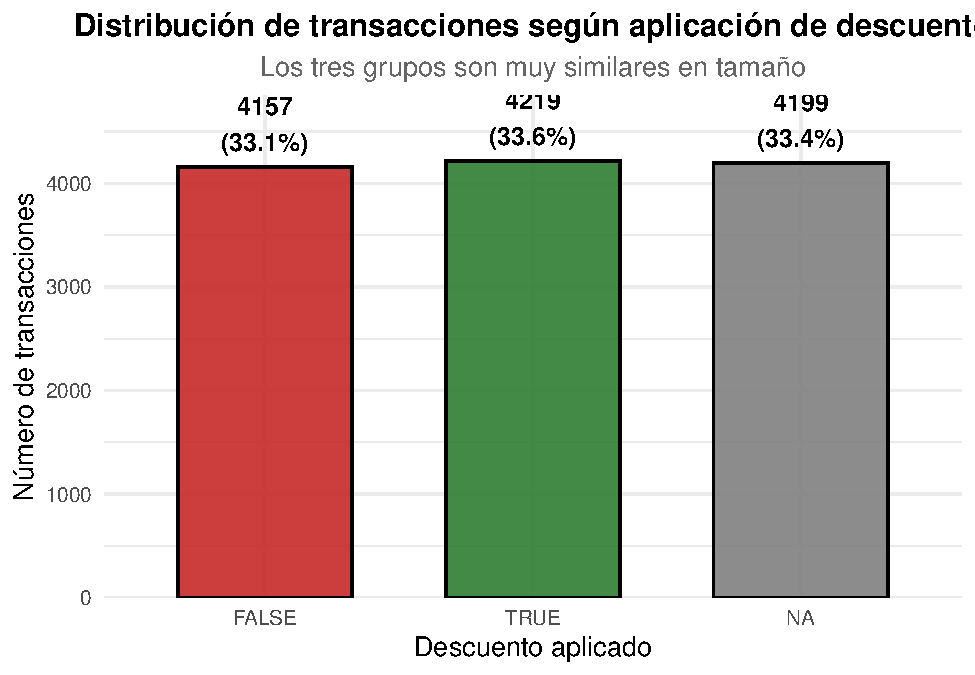
\includegraphics[width=0.9\linewidth,]{informe_files/figure-latex/unnamed-chunk-15-1} \end{center}

\begingroup\fontsize{12}{14}\selectfont

\begin{longtable}[t]{cccccccc}
\caption{\label{tab:unnamed-chunk-16}Medidas de resumen de Total Spent y Quantity según Descuento}\\
\toprule
Descuento & N & Media Total & Mediana Total & Desv. Total & Media Cantidad & Mediana Cantidad & Desv. Cantidad\\
\midrule
FALSE & 4157 & 129.95 & 109.5 & 93.35 & 5.58 & 6 & 2.85\\
TRUE & 4219 & 130.49 & 109.5 & 95.54 & 5.53 & 6 & 2.85\\
NA & 4199 & 128.51 & 105.0 & 95.35 & 5.49 & 6 & 2.88\\
\bottomrule
\end{longtable}
\endgroup{}

\begin{center}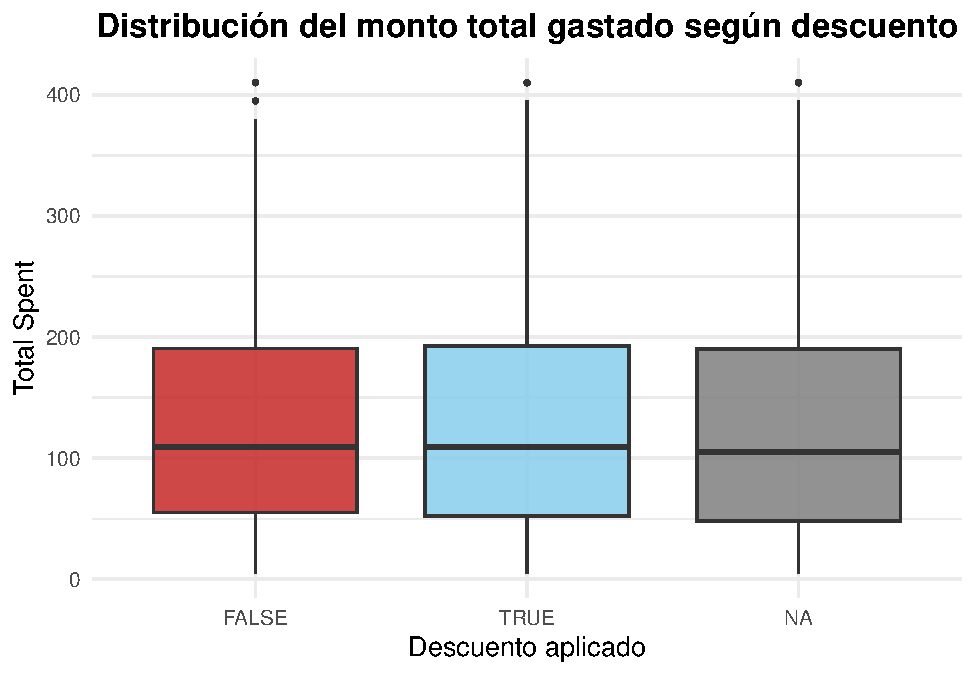
\includegraphics[width=0.9\linewidth,]{informe_files/figure-latex/unnamed-chunk-17-1} \end{center}

\begin{center}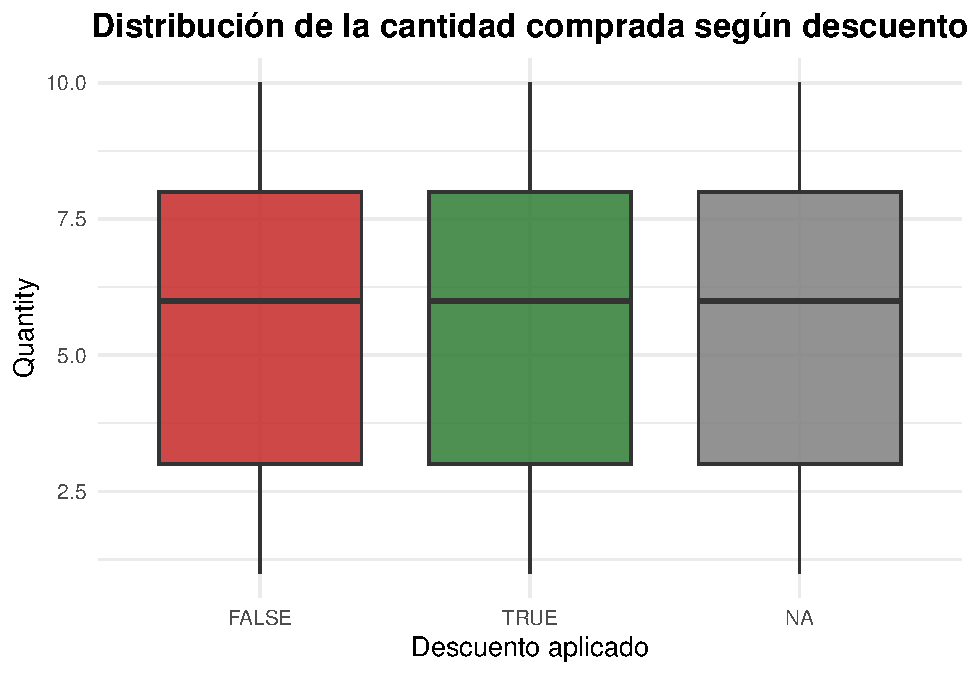
\includegraphics[width=0.9\linewidth,]{informe_files/figure-latex/unnamed-chunk-18-1} \end{center}

\begingroup\fontsize{11}{13}\selectfont

\begin{longtable}[t]{cccc}
\caption{\label{tab:unnamed-chunk-19}Distribucion de descuentos segun categoria (solo TRUE y FALSE)}\\
\toprule
Categoria & Descuento & Frecuencia & Porcentaje (\%)\\
\midrule
Beverages & FALSE & 495 & 48.7\\
Beverages & TRUE & 521 & 51.3\\
Butchers & FALSE & 514 & 48.6\\
Butchers & TRUE & 543 & 51.4\\
Computers and electric accessories & FALSE & 546 & 50.5\\
\addlinespace
Computers and electric accessories & TRUE & 535 & 49.5\\
Electric household essentials & FALSE & 528 & 50.3\\
Electric household essentials & TRUE & 522 & 49.7\\
Food & FALSE & 547 & 51.8\\
Food & TRUE & 508 & 48.2\\
\addlinespace
Furniture & FALSE & 486 & 47.6\\
Furniture & TRUE & 535 & 52.4\\
Milk Products & FALSE & 549 & 50.4\\
Milk Products & TRUE & 540 & 49.6\\
Patisserie & FALSE & 492 & 48.9\\
\addlinespace
Patisserie & TRUE & 515 & 51.1\\
\bottomrule
\end{longtable}
\endgroup{}

\begin{center}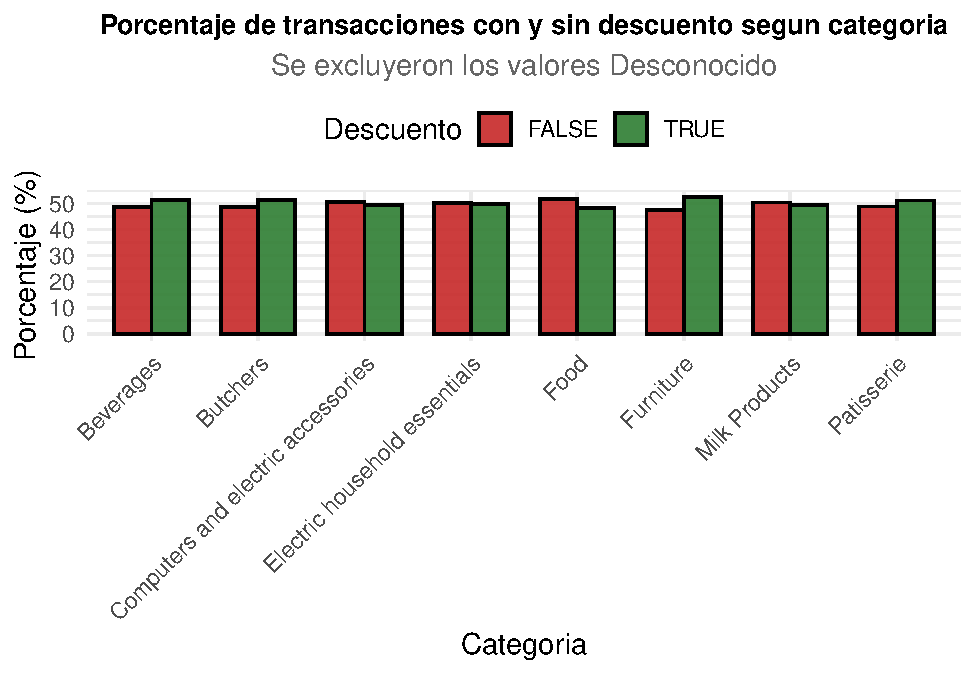
\includegraphics[width=0.9\linewidth,]{informe_files/figure-latex/unnamed-chunk-20-1} \end{center}

\begin{longtable}[t]{cccc}
\caption{\label{tab:unnamed-chunk-21}Distribucion de descuentos segun canal de venta (Online vs In-store)}\\
\toprule
Location & Descuento & Frecuencia & Porcentaje (\%)\\
\midrule
In-store & FALSE & 2055 & 49.8\\
In-store & TRUE & 2070 & 50.2\\
Online & FALSE & 2102 & 49.4\\
Online & TRUE & 2149 & 50.6\\
\bottomrule
\end{longtable}

\begin{center}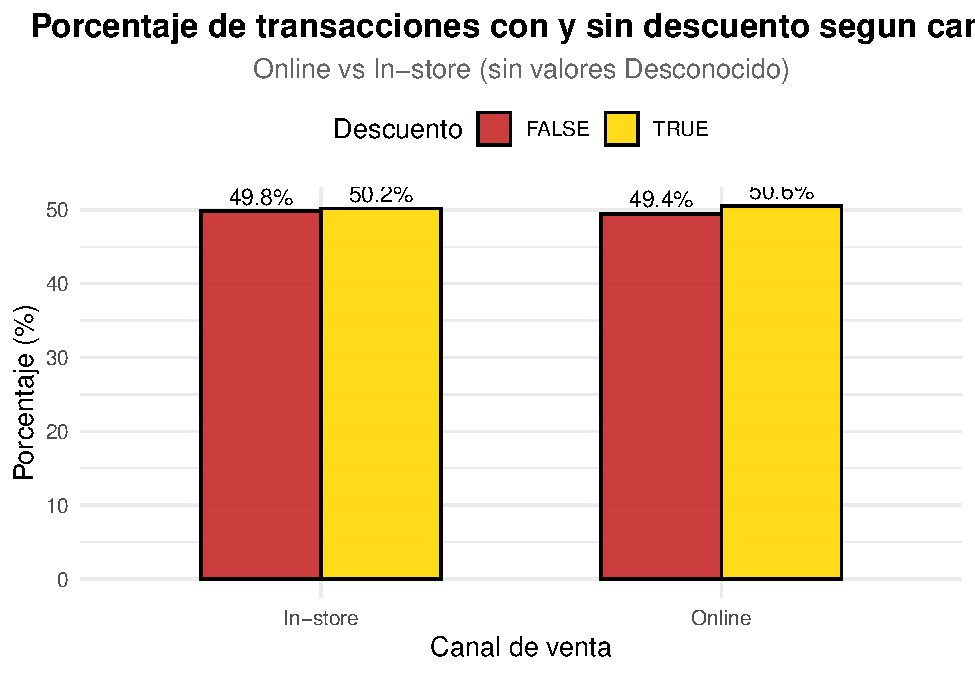
\includegraphics[width=0.9\linewidth,]{informe_files/figure-latex/unnamed-chunk-22-1} \end{center}

\begingroup\fontsize{11}{13}\selectfont

\begin{longtable}[t]{cccc}
\caption{\label{tab:unnamed-chunk-23}Distribucion de descuentos segun metodo de pago}\\
\toprule
Metodo de Pago & Descuento & Frecuencia & Porcentaje (\%)\\
\midrule
Cash & FALSE & 1378 & 48.6\\
Cash & TRUE & 1459 & 51.4\\
Credit Card & FALSE & 1359 & 49.3\\
Credit Card & TRUE & 1397 & 50.7\\
Digital Wallet & FALSE & 1420 & 51.0\\
\addlinespace
Digital Wallet & TRUE & 1363 & 49.0\\
\bottomrule
\end{longtable}
\endgroup{}

\begin{center}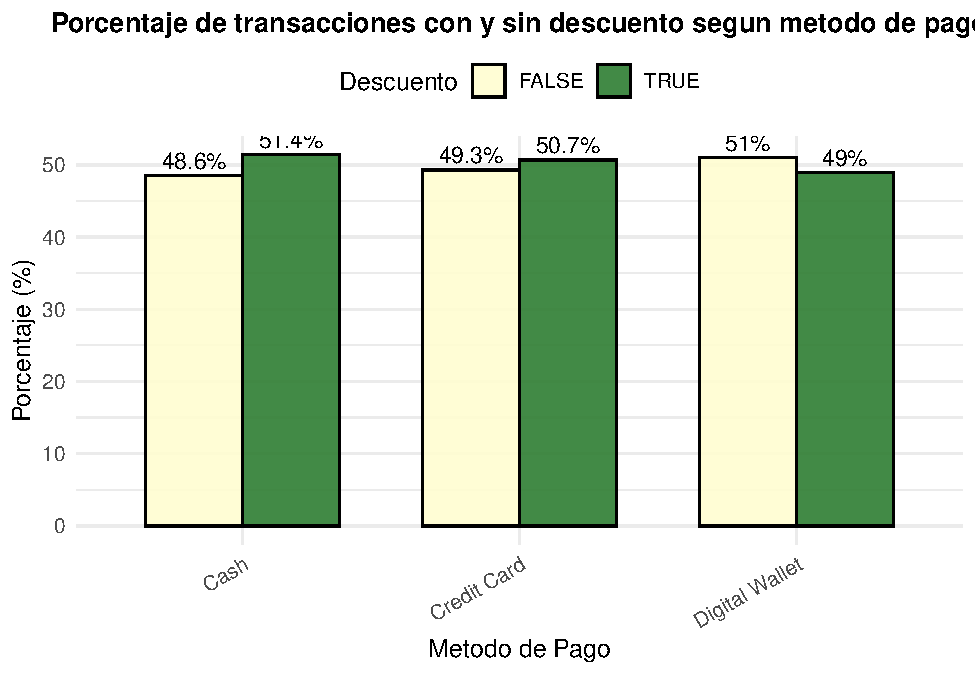
\includegraphics[width=0.9\linewidth,]{informe_files/figure-latex/unnamed-chunk-24-1} \end{center}

\begin{longtable}[t]{ccccc}
\caption{\label{tab:unnamed-chunk-25}Ticket promedio (Total Spent) segun metodo de pago y descuento}\\
\toprule
Metodo de Pago & Descuento & N & Media & Mediana\\
\midrule
Cash & FALSE & 1378 & 131.24 & 111.0\\
Cash & TRUE & 1459 & 134.06 & 110.0\\
Credit Card & FALSE & 1359 & 132.84 & 112.0\\
Credit Card & TRUE & 1397 & 127.56 & 107.5\\
Digital Wallet & FALSE & 1420 & 125.90 & 102.0\\
\addlinespace
Digital Wallet & TRUE & 1363 & 129.68 & 108.0\\
\bottomrule
\end{longtable}

\begin{center}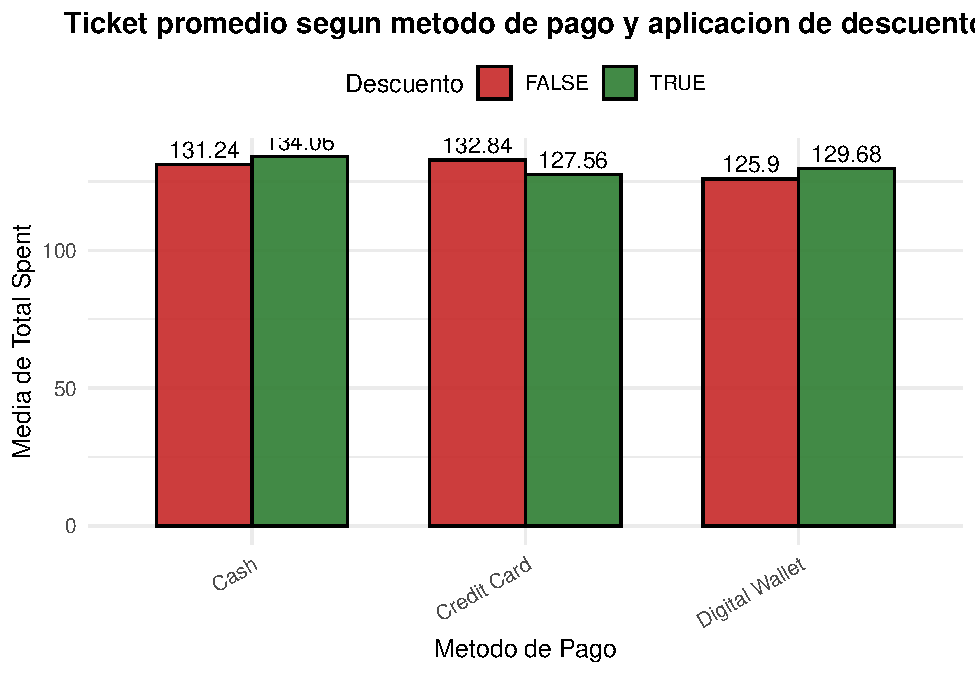
\includegraphics[width=0.9\linewidth,]{informe_files/figure-latex/unnamed-chunk-26-1} \end{center}

\{\small Este capítulo presenta los resultados obtenidos al aplicar las
metodologías descritas en el capítulo anterior, así como del análisis
estadístico descriptivo de las variables estudiadas y las ventajas y
desventajas al aplicar dichos tests.\}

\section{Presentación de resultados 1}

Descripción\\

\section{Presentación de resultados 2}

Descripción\\

\section{Presentación de resultados n}

Descripción\\

\chapter{Conclusiones y Recomendaciones}

\textbf{1.-} Conclusion 1 del trabajo de investigación.\\

\textbf{Recomendación} Recomendación 1 del trabajo de investigación.\\

\textbf{2.-} Conclusion 2 del trabajo de investigación.\\

\textbf{Recomendación} Recomendación 2 del trabajo de investigación.\\

\textbf{n.-} Conclusion n del trabajo de investigación.\\

\textbf{Recomendación} Recomendación n del trabajo de investigación.\\

\appendix
\renewcommand{\thechapter}{\Alph{chapter}}

\chapter{Anexo A}

\chapter{Anexo B}

\chapter{Anexo C}

%%%%%%%%%%%%%%%%%%%%%%%%%%%%%%%%%%%%%%%%%%%%%%%%%%%%%
%                   REFERENCIAS                     %
%%%%%%%%%%%%%%%%%%%%%%%%%%%%%%%%%%%%%%%%%%%%%%%%%%%%%
% Mantenemos la estructura natbib de tu plantilla
\renewcommand{\bibname}{Lista de Referencias}
\bibliographystyle{apalike} 
\bibliography{bibliografia.bib} 

%%%%%%%%%%%%%%%%%%%%%%%%%%%%%%%%%%%%%%%%%%%%%%%%%%%%%
%                   APÉNDICES                       %
%%%%%%%%%%%%%%%%%%%%%%%%%%%%%%%%%%%%%%%%%%%%%%%%%%%%%

\end{document}
